\documentclass[runningheads]{llncs}
%
\usepackage{graphicx}
\usepackage{algpseudocode,algorithm}
\usepackage{hyperref}
\usepackage{listings}
\usepackage{xcolor}
\usepackage{xstring}
\usepackage[nointegrals]{wasysym}
\usepackage{MnSymbol}
\usepackage{booktabs} % For formal tables
\graphicspath{ {../images/} }

\definecolor{NavyBlue}{HTML}{000080}
\definecolor{Magenta}{HTML}{FF00FF}
\definecolor{Orange}{HTML}{FFA500}
\definecolor{CornflowerBlue}{HTML}{6495ED}
\definecolor{YellowGreen}{HTML}{9ACD32}
\definecolor{Gray}{HTML}{BEBEBE}
\definecolor{Yellow}{HTML}{FFFF00}
\definecolor{GreenYellow}{HTML}{ADFF2F}
\definecolor{ForestGreen}{HTML}{228B22}
\definecolor{Lavender}{HTML}{FFC0CB}
\definecolor{SkyBlue}{HTML}{87CEEB}
\definecolor{NavyBlue}{HTML}{000080}
\definecolor{Goldenrod}{HTML}{DDF700}
\definecolor{VioletRed}{HTML}{D02090}
\definecolor{CornflowerBlue}{HTML}{6495ED}
\definecolor{LimeGreen}{HTML}{32CD32}


% Used for displaying a sample figure. If possible, figure files should
% be included in EPS format.
%
% If you use the hyperref package, please uncomment the following line
% to display URLs in blue roman font according to Springer's eBook style:
% \renewcommand\UrlFont{\color{blue}\rmfamily}

\begin{document}
%
\title{Event-driven multi-population optimization: mixing Swarm and Evolutionary strategies}
%
%\titlerunning{Abbreviated paper title}
% If the paper title is too long for the running head, you can set
% an abbreviated paper title here
%
\author{First Author\inst{1}\orcidID{0000-1111-2222-3333} \and
Second Author\inst{2,3}\orcidID{1111-2222-3333-4444} \and
Third Author\inst{3}\orcidID{2222--3333-4444-5555}}
%
\authorrunning{F. Author et al.}
% First names are abbreviated in the running head.
% If there are more than two authors, 'et al.' is used.
%
\institute{Princeton University, Princeton NJ 08544, USA \and
Springer Heidelberg, Tiergartenstr. 17, 69121 Heidelberg, Germany
\email{lncs@springer.com}\\
\url{http://www.springer.com/gp/computer-science/lncs} \and
ABC Institute, Rupert-Karls-University Heidelberg, Heidelberg, Germany\\
\email{\{abc,lncs\}@uni-heidelberg.de}}
%
\maketitle              % typeset the header of the contribution
%
\begin{abstract}
    Recently, in the field of nature-inspired optimization,
researchers have proposed multi-population asynchronous algorithms
that distribute the evolutionary process among heterogeneous search
paradigms. These algorithms execute the search strategy by reading
streams of populations from message queues, and replacing them with
evolved versions of them.  Moreover, current studies suggest that when
we have a high number of populations interacting in parallel, the
effect of the individual parameters of each population is compensated
by those selected in other populations, improving the overall
performance of the algorithm. In this work, we propose a simple
reactive migration method for the asynchronous execution of
multi-population, multi-strategy algorithms that improves over
homogeneous configurations.  We evaluate this method by comparing with
homogeneous and an ensemble of multi-populations, using Genetic
Algorithms (GAs) and Particle Swarm Optimization (PSO) in the
noiseless BBOB testbed for the optimization of continuous
functions. Results show, that this method offers better performance,
even when compared with other asynchronous population based
algorithms.
\keywords{heterogeneous multi-population algorithms  \and genetic algorithms
 \and cloud-native systems.}
\end{abstract}
%
%
%
\section{Introduction}

Nature-inspired optimization algorithms have been used successfully in the last
decades to tackle complex problems \cite{yang2014nature}. These
algorithms include evolutionary algorithms (EAs)
\cite{back1996evolutionary} and swarm intelligence (SI)
\cite{kennedy2006swarm}. 
Genetic Algorithms (GAs) 
\cite{holland1992adaptation,eiben2003genetic}, 
Differential Evolution (DE) \cite{karabouga2004simple}, and 
Genetic Programming (GP) \cite{back1996evolutionary} are popular EAs, while examples of SI algorithms 
\cite{kennedy2006swarm} are particle swarm optimization (PSO)
\cite{clerc2010particle}, artificial bee colony (ABC) \cite{karaboga2005idea}, Grey Wolf Optimization
(GWO) \cite{mirjalili2014grey}, and ant colony algorithms (ACO) \cite{dorigo1999ant}.
A common characteristic of these kind of methods is the
use of an initial set of random candidate solutions that are manipulated by the
algorithm to generate a new set of candidates, and because of this, we commonly
referred to them as population-based algorithms. 
There are other stochastic optimization methods, that even if they are not
nature-inspired, they employ the concept of an evolving population. An example
of this kind of methods is population-based incremental learning (PBIL)
\cite{baluja1994population}, which is an optimization and an estimation of
distribution algorithm. Since instead of piecewise constructing a population or changing it
incrementally, all members of the population have to be evaluated to
obtain a fitness or score that will be used to select them (or not), a
drawback of this kind of algorithms is that they can be computationally
expensive since it is difficult to overcome that $n$ factor, where $n$
is the population size, in the complexity of every iteration of the
algorithm. That is why researchers have been proposing some form of
parallelization since early on \cite{muhlenbein1988evolution} with 
the goal of decreasing their execution time. % Not scalability, but wallclock timing - JJ
One of the first methods of parallelization was the island
model, which lead to an increased performance
\cite{gorges1990explicit,grosso1985computer}. The concept was to divide the
population into smaller populations that communicated with each other. Other
population-based algorithms have adopted the technique, and since then,
researchers have found additional advantages besides a reduced execution speed, 
these include avoiding a premature convergence and maintaining the diversity of the
global population \cite{li2015multi}, we are going to call these methods 
multi-population algorithms \cite{Ma2019}. The relative 
isolation in which populations carry out the algorithm, together with the
synchronous or asynchronous communication, helps to increase the overall
diversity since each population will search in a particular area, at least
between communications. Multi-population algorithms use a form of
communication to recombine or migrate candidate solutions between populations
to avoid premature convergence, since smaller populations are known to perform
better for a given problem than bigger populations
\cite{li2016multi,wu2016differential}. Even in some cases, a multi-population based
algorithm scales better due to these interactions, and the parallelism of the
operation \cite{ALBA20027}. 

Having many populations offers researchers many configuration options and
additional challenges when designing efficient multi-population algorithms.
Options include the number and size of populations, the interaction between
them, the search area of each population, and the search strategy and its
parametrization for each population.  In this paper, we are interested in the
latter, that is, having multiple populations running with distinct parameters
and optimization algorithms. We can find in the literature, several
heterogeneous multi-population algorithms that integrate variations of optimization
algorithms, and these often perform better than single-population or homogeneous
multi-population optimization algorithms\cite{wu2016differential,nseef2016adaptive}.
Heterogeneous algorithms add to
the problem of finding the correct parameter settings for each population;
because some parameters affect the accuracy of the solution and the convergence
speed of the individual algorithms as they tip the balance between exploration
and exploitation of the search space. On the other hand, current studies show
that by having a high number of populations communicating in parallel, the
effect of the individual parameters of each population is compensated by those
selected in other populations \cite{li2016multi,tanabe2013evaluation}. Some
level of heterogeneity can be implemented by just changing the configuration
parameters of each population, but in this case, we are interested in
heterogeneous search strategies.

Therefore, in this paper, we implemented an asynchronous multi-population
algorithm version, using a message queue for inter-process communication 
\cite{guervos2018introducing}, and a reactive migration procedure, in which we compare
three heterogeneous configurations using a randomized parameter technique. We
experimented with all populations using a GA or PSO search strategies, versus an
ensemble multi-population with both GA and PSO algorithms, using as a benchmark,
the separable functions of the BBOB noiseless testbed \cite{hansen2009real}. 
We compare the options by
measuring the average running time (aRT) as the number of functions (\#FEs), as
the objective is to prove that the advantage of heterogeneous configurations
resides not only in the increased scalability but also in the search
performance. 

The organization of the paper is as follows: First, Section \ref{soa} presents
state of the art relevant to our work. In Section \ref{method}, we present the
proposed method.  Section \ref{setup} describes the design of the empirical
evaluation we designed to assess the effectiveness of the method, and in Section
\ref{results}, we report and discuss the results. Finally, we offer the
conclusions of this paper and suggestions on future work in Section
\ref{conclusions}.


\section{State of the Art}
\label{soa}

In general, population based algorithms have to keep a balance between
exploration and exploitation via the clever use of selection and
variation operators \cite{vcrepinvsek2013exploration}. In pursuit of
that objective, it is important to keep diversity high
\cite{yuan2005importance}, but different algorithms have different
mechanisms for increasing diversity (exploration) or decreasing it
(exploitation). PSO has two constants that rule in which direction the
{\em particle} is going to move: either randomly (exploration) or in
the direction of the best particle (exploitation); evolutionary
algorithms use mutation and, to a certain point, crossover for
exploration and crossover and selection procedures for
exploitation. Since these mechanisms are fundamentally different,
using several different algorithms at the same time might be
considered a win-win situation by way of performing exploitation in
several different directions at the same time, which will be able to
get closer to the solution as well as generate new possibilities.

This
is why hybrid population-based algorithms have been repeatedly
suggested in the literature: Pandi et al. \cite{pandi2011dynamic}
suggest a combination of swarm intelligence and another algorithm
denominated harmony search; Lien et al. \cite{lien2012hybrid} combine
particle swarm optimization with bee colony algorithms, while Zhao et
al. \cite{zhao2010hybrid} combine the latter with evolutionary
algorithms.

\begin{table}[h!tb]
    \caption{Equivalence of terms between particle swarm optimization
    and evolutionary algorithms. \label{tab:equivalence}}
\centering
\begin{tabular}{|c|c|}
  \hline
  PSO & EA \\ \hline
  Position vector & {\em genes} in a chromosome \\ \hline
  Move towards better & Selection  \\ \hline
  Random motion & Mutation \\ \hline
  Move towards centroid & Crossover \\ \hline
\end{tabular}
\end{table}
%
EAs and PSOs share another characteristic, besides the fact that they
act on populations: they can use the same data structures to
represent every member of the population. Please check Table
\ref{tab:equivalence} for equivalence of terms between PSO and EAs;
additionally to the data structures used, there is a certain
equivalence in the operators, but they are different enough to perform
search in different ways. The fact that they use the same data
structures means that you can apply them in turns, or simply start
calling a ``chromosome'' a ``particle'' or the other way round,
without any conversion, and keep working with it.

This is what the first papers to propose such a hybrid algorithm, by
Robinson et al. \cite{Robinson2002}, explicitly played on this
fact and also on what we might call diversity of local minima by
running an algorithm on a population until it became stagnated, and
then switching to the other one. This was done apparently only once,
but eventually the mixture of the two algorithms was able to obtain
better results in the design of a kind of antenna called ``horn'' than
each one of them separately, although they report that the best value
was obtained by the algorithm that started as a PSO and terminated as
an evolutionary one.

Another kind of hybrid was proposed independently by 
Shi et al. \cite{shi2003hybrid}, citing the ``local optimum'' problem,
that is, the same as the previous one; it mixes both algorithms
testing in different configurations: ``parallel'' and ``serial''
testing which configuration works better and is able to avoid
that. Their results on benchmark functions are mixed;
In general, however, a well-designed evolutionary or PSO
algorithm will not fall in that local optimum; it is certainly true
that, within a certain evaluation budget, neither might be able to
find that global optimum. However, it is probably that they mean that,
since exploitation of better-than-average solutions is done by the two
algorithms in different directions, a hybrid algorithm might help the
single-algorithm version to escape that.

This better exploitation capability was used by Grimaldi et al.
\cite{grimaldi2005genetical}, with the objective of solving electromagnetic problems. What they do is
to split the population into two different populations which will be
processed by an EA and a PSO algorithm; the new individuals generated
are merged in a single population, which is then split all over again
in the next iteration. This guarantees that none of the two algorithms
is getting stuck, since the individuals will be randomly subjected to
one or the other on every generation.


\begin{figure*}[h!tb]
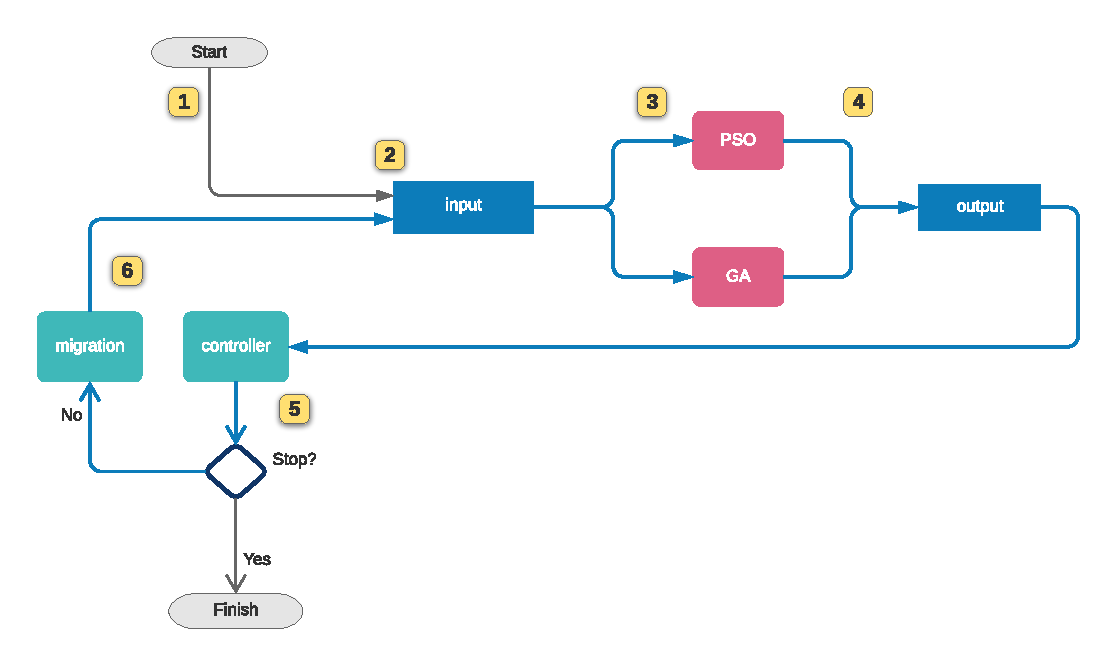
\includegraphics[width=5in]{../images/kafkeo}
\caption{General scheme of the architecture of this method. Numbers will be used to refer to its different elements in text.}
\label{fig:kafkeo}
\end{figure*}
%
Later on, Esmin et al. \cite{esmin2006hybrid} leveraged to design their
algorithms; this idea was
later extended by Li et al. \cite{li2008gene}; in this work,
chromosomes/particles represent Support Vector Machines, which are
optimized to find the most representative features of gene expression
data sets. PSO and EAs are applied serially: 10 iterations of each,
after which the finalization criterion is examined; first PSO, then
EA. Separate EA and PSO are tested against this hybrid algorithm,
finding improvements of a few percent points in the accuracy over
classification of the whole dataset. This marginal, but significant,
improvement is essentially the kind of results that should be
expected. While improvements in diversity always boost the results by
allowing the algorithms to find better solutions, an
order-of-magnitude difference is not usually  achieved, since both
algorithm, by themselves, have good mechanisms for global
exploration.

Several other hybrid algorithms have been proposed more recently:
Gulia et al. \cite{gulia2019hybrid} mix ant colony optimization, 
which is a swarm intelligence algorithm, and EAs to select
software testing cases. ACO and EA are used serially, with GA acting
to refine the test suite initially selected by the ant algorithm.

The state of the art is, then, use swarm intelligence and evolutionary
algorithms coupled to a population to which they are applied either
one after the other, or splitting the population so that every one is
applied to a part. In our case, however, population and algorithms are
decoupled, and this decoupled architecture allows to mix algorithms in
several different ways, which will be tested in this paper using the
method explained next.


\section{Proposed Method}
\label{method}
%
% 
% Write a small introduction here - JJ
% done - Mario 
In this section, we present a model for the execution of multi-population based
asynchronous algorithms. As a first step, we describe the general architecture,
for handling a stream of continuously updated populations,  and then our
approach for decoupling the processing in stateless functions, to finally give
details of the migration mechanism.


\subsection{Architecture}
\label{arch}

In this section we present our proposed model for the execution of
multi-population based asynchronous algorithms. As we have mentioned before, when
designing efficient multi-population algorithms, we need to consider additional
issues \cite{Ma2019}, including the number and size of populations, how they
interact or communicate between them, and the search strategy and parametrization of
populations. We have considered these requirements and, in this paper,
propose a cloud-native
multi-population solution. In this model, populations are the primary data
structure, and we package them as messages that are part of a continuous stream flowing
from one computing node, performing an algorithm, to the next. To achieve this ``continuous stream,''
everything must happen asynchronously without computing nodes needing to wait for
others, and becoming available as soon as it is needed.

We have implemented this streaming functionality by using a message queue
system, whose general architecture is shown in Figure \ref{fig:kafkeo}. We can explain
the model by using an analogy of producers and consumers of messages. There are
two queues, one labeled \texttt{input}, and the other one \texttt{output}. In a
queue, {\em push} operations are represented by solid arrows connecting to the
left side and pull or pop operations as solid arrows leaving from the right
side. The \texttt{controller} process, is responsible for the migration of
individuals from one population to the other, and keeping track of the
iterations of the algorithm. There is at least one \texttt{stateless function}
worker process responsible for running the isolated algorithms. The two
processes \texttt{PSO} and \texttt{GA}, are shown.

We can follow the path of messages as follows:

\begin{enumerate}

\item In this step, the specified number of populations are created according
to the configuration. Populations at this moment are just static data messages,
including each individual inside. Each population includes a metadata section
where its algorithm and execution parameters are specified. For instance, for a
GA, the mutation rate, type of crossover operator, and other values are
indicated.

\item The setup process pushes each population on to the \texttt{input}
queue so that they can be consumed by stateless functions responsible for the
execution of the search.

% before you have used Function in caps - JJ - corrected - Mario
\item One or more \texttt{stateless functions} are constantly pulling
population messages from the \texttt{input} queue. These functions have the
task of executing the optimization algorithm. They take the current state of
the population and start to run the specified algorithm for a certain number of
iterations.

\item Once they finish the execution, the resulting populations are pushed to
the \texttt{output} queue; when the computing node is done with a population, it draws another one from the
queue.

% You are using also caps here for the queue name - JJ  - corrected - Mario
\item The \texttt{controller} pulls populations from the \texttt{output} queue,
inspects the metadata describing the current state of the populations, and if
the algorithm has found an optimal solution or the maximum number of iteration
has been reached it stops the execution.

\item Otherwise, it passes the stream of messages to a migration function,
where populations are mixed. Migration generates new populations, and they are
again pushed to the \texttt{input} queue to continue in a loop. The
\texttt{controller} is also responsible for logging the metadata.

\end{enumerate}

This reactive architecture has the following advantages:
\begin{itemize}

\item It decouples the population and the population-based algorithm. In this
design, we can have one or many processing nodes, each running a different
search strategy.

\item Also, the reactive controller gives designers more control over the
multi-population algorithm. In this process, designers can dynamically change
the number of populations, population parameters, and migration details
on-the-fly.

\item Another advantage is that algorithm designers have many options for
implementing this simple architecture. The same basic components can be
implemented as a single multi-threaded program, or as a highly scalable
serverless cloud application.
\end{itemize}

\subsection{Stateless functions} 
\label{functions} 

% Maybe mention that before? You have already mentioned them above - JJ
This message queue pattern is an essential component of a highly scalable
reactive architecture; one of the reasons for this scalability is the use of
stateless functions that have no secondary effects, or the need to read data
from an external entity. Stateless functions do not need to read, keep, or
modify data outside of the scope of the method, it will have no side
effects reading inputs and producing an output, mapping input to output
as it were. If we implement population-based
optimization algorithms using stateless functions, then to the system, there is
no difference between having one or many copies of the same function pulling
work from the queue all at the same time, because there are no unwanted side
effects, including problems of resource locking resulting from this
concurrency. This architecture has been implemented successfully for 
developing cloud-native multi-population algorithms,
using serverless functions \cite{garcia2018modern}, and concurrent programming \cite{guervos2019improving}.  
% Add a few references to our papers, anonymized or not - JJ

To have a stateless version of a population-based algorithm, we only need to
skip the step of creating a random population. Instead, the function receives
the population as a parameter along with the required parameters. After several
iterations (specified in the parameters), the function returns the current state
of the population, with additional data describing the local execution. This
data is necessary to log the \#FE and current fitness values.


\subsection{Migration}
\label{migration}

As the controller is pulling population messages from the output queue, it waits
until the message queue contains three valid populations to trigger an event handled by the
\texttt{population\_mixer} function, which uses as an argument a list
containing the three populations. This design has the advantage of not needing to keep a
buffer in memory or external storage, and it follows the reactive paradigm. A
possible disadvantage can be that it only mixes populations that have
arrived sequentially to the message queue, but we
could mitigate this with a larger buffer and in fact populations do
not need to arrive to the buffer in the same order they were created
or processed, so this shouldn't, in principle, contribute to any loss
of diversity.

When \texttt{population\_mixer} unit receives a list of three populations, let us say
[A, B, C], it calls the migration method shown in Algorithm \ref{alg:migration}
for [A, B], [B, C] and [A, C]. The migration algorithm sorts the
individuals of each population and generates a new one by
merging the best half from each. Finally, the \texttt{population\_mixer} 
method pushes the three generated populations back to the \texttt{input} message queue.

\begin{algorithm}
    \caption{Migration}
    \label{alg:migration}
    \begin{algorithmic}[1]
        \Procedure{cxBestFromEach}{$pop_1,pop_2$}
            \State $pop_1.sort()$
            \State $pop_2.sort()$
            \State $size\gets min(len(pop_1), len(pop_2))$
            \State $cxpoint\gets (size-1)/2$
            \State $pop_1[cxpoint:]\gets pop_2[:cxpoint+2]$
            \State \textbf{return} $pop_1$
        \EndProcedure 
    \end{algorithmic}
\end{algorithm}
%
\begin{figure}[h!tb]
  \begin{tabular}
      {c@{\hspace*{-0.00001\textwidth}}
      % c@{\hspace*{-0.00001\textwidth}}
      }
     
  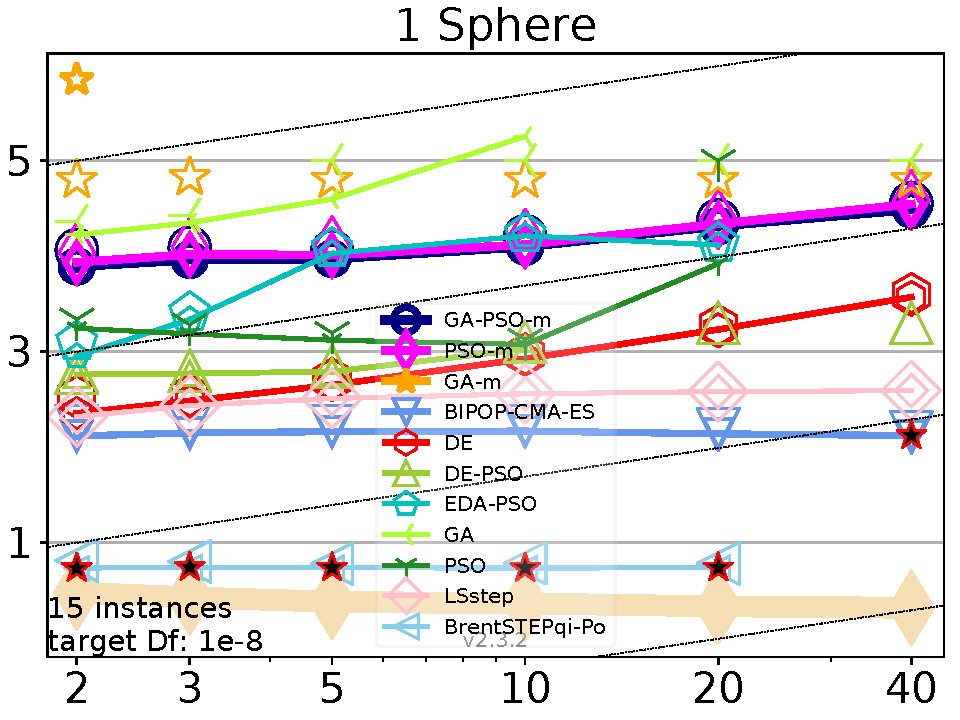
\includegraphics[width=0.30\textwidth]{ppfigs_f001}
  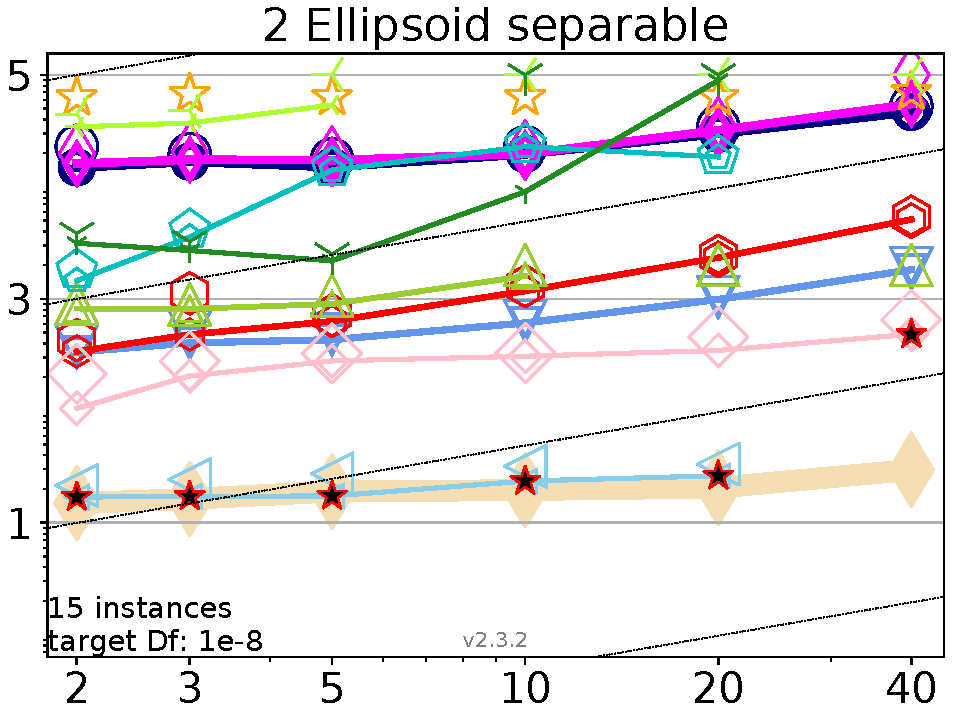
\includegraphics[width=0.30\textwidth]{ppfigs_f002}

  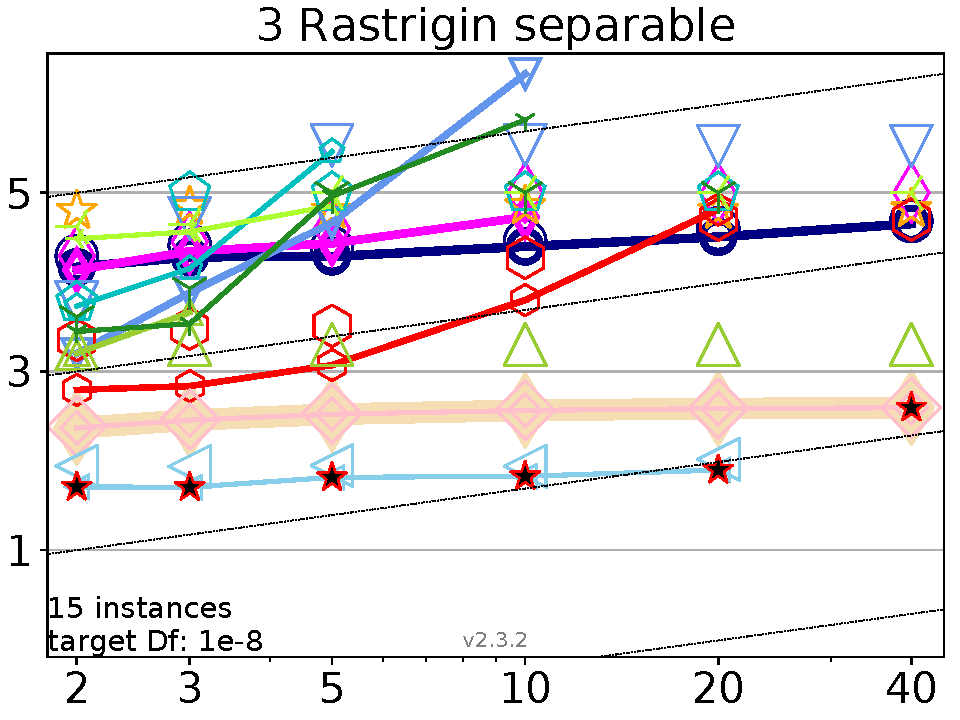
\includegraphics[width=0.30\textwidth]{ppfigs_f003}\\
  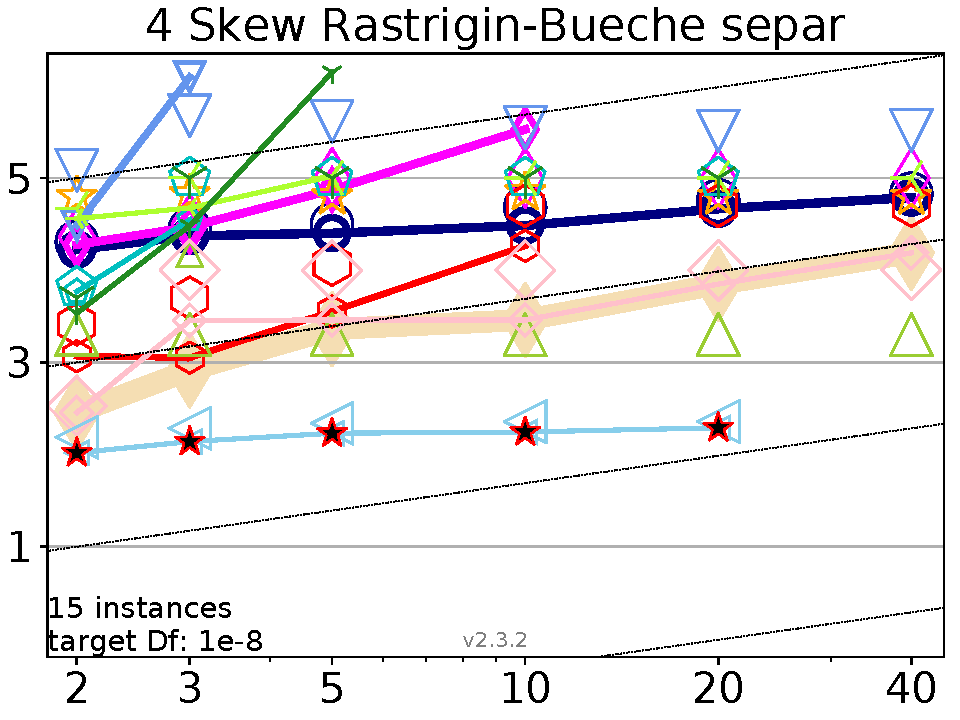
\includegraphics[width=0.30\textwidth]{ppfigs_f004}
  
  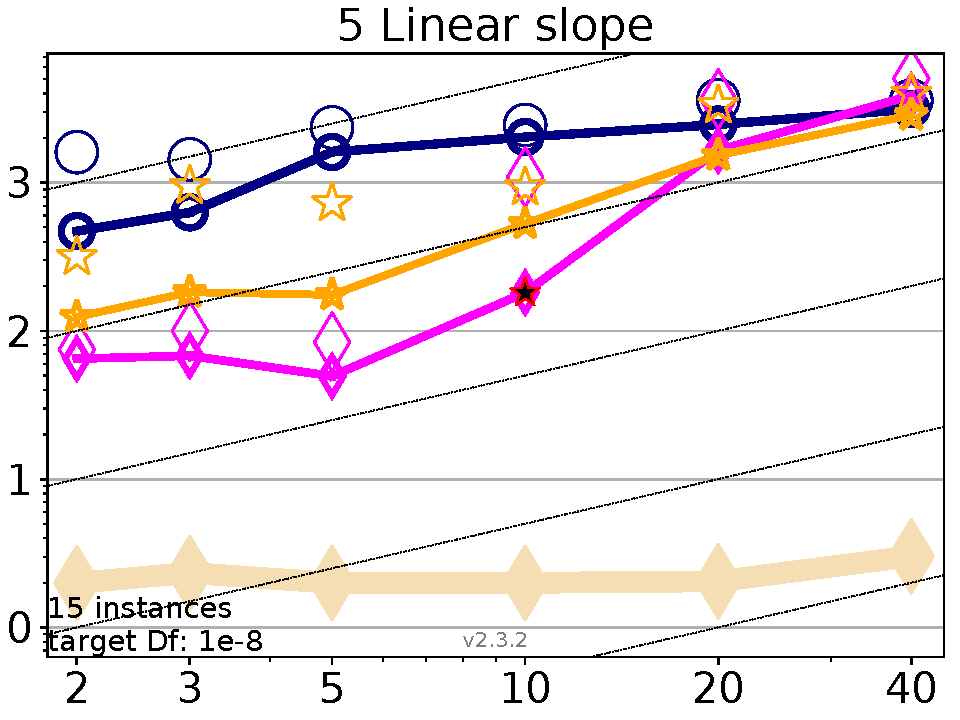
\includegraphics[width=0.30\textwidth]{ppfigs_f005}
  \end{tabular}
  \vspace{-3ex}
   \caption{Average running time (in \#FEs as $log_{10}$ value),
    divided by dimension for target function value $10^{-8}$ vs dimension. 
    Black stars indicate a statistically better result compared to 
    all other algorithms ($p < 0.01$) and Bonferroni 
    correction number of dimensions. 
    Legend: {\color{NavyBlue}$\circ$}:GA-PSO-m, 
    {\color{Magenta}$\diamondsuit$}:PSO-m, 
    {\color{Orange}$\star$}:GA-m, 
    {\color{CornflowerBlue}$\triangledown$}:BIPOP-CMA-ES,
    {\color{red}$\varhexagon$}:DE, 
    {\color{YellowGreen}$\triangle$}:DE-PSO, 
    {\color{cyan}$\pentagon$}:EDA-PSO, 
    {\color{GreenYellow}$\rightY$}:GA, 
    {\color{ForestGreen}$\downY$}:PSO, 
    {\color{Lavender}$\Diamond$}:LSstep, 
    {\color{SkyBlue}$\triangleleft$}:BrentSTEP
    } 
  \label{fig:avg}
\end{figure}
%
\section{Experimental setup}
\label{setup}

In this section, we present the experimental setup needed 
to verify if having a multi-population algorithm, with
heterogeneous populations and the support for mixing search strategies,
increases the performance of the search by needing fewer function evaluations
than a homogeneous setting.

% Use present perfect more than past - JJ For the experiment, we have used five
benchmark separable functions ($f_1 to f_5 $) from the Continuous Noiseless
BBOB testbed, which is part of the Comparing Continuous Optimizers (COCO)
framework \cite{hansen2016coco}. 

Although there are not many real-world
problems that are entirely separable, we wanted to focus on separable functions
as a primary benchmark for testing the performance of a hybrid multi-population
algorithm. And there is interest in solving such problems using more
general methods \cite{doerr2013evolutionary,swarzberg1994step}. % Say why only 5, and these 5 - JJ 

These functions are real-parameter, single-objective, and are
usually employed as benchmarks. We have tested with fifteen instances of each
function, each one having a different optimal value. The standard benchmark of
the testbed % which testbed? uses these 15 instances over 2, 3, 5, 10, 20, and
40 dimensions. With the maximum number of function evaluations (\#FEs)
increasing with the dimension (D), using the expression $10^5 \cdot D$ (i.e.
for $D = 2$, \#FEs is $200,000$).

The COCO framework offers several tools to compare the performance of
algorithms, generating data sets, tables, and reports for an experiment, we have
compared using the average required time (aRT). There is a
repository\footnote{\url{https://coco.gforge.inria.fr/doku.php?id=algorithms-bbob}}
of more than 200 results for the noiseless BBOB testbed, collected from BBOB
workshops and special sessions between the years 2009 and 2019. To test the
heterogeneous multi-population capabilities, we have compared the aRT between a
homogeneous and an ensemble of multi-populations, using Genetic Algorithms
(GAs) and Particle Swarm Optimization (PSO).

We have used the DEAP framework for the
GA stateless function \cite{fortin2012deap} and the EvoloPy library
\cite{faris2016evolopy} for the PSO algorithm function. We show the parameters
for each algorithm in Tables \ref{tab:GAparams} and Table \ref{tab:PSOparams}
for the GA and PSO, respectively. We have obtained these parameters by following a
method used by García et al. in \cite{garcia2017benchmarking}. First, we
tested the parameters for the Rastrigin separable function with five
dimensions. After about fifteen experiments, the most challenging targets were
achieved for this particular function. We tested again with functions one to
three, and after obtaining favorable results, we set the PSO and GA algorithm
parameters. We have set the mutation and crossover probabilities of the GA randomly
to have heterogeneous populations; the entry in the Table shows the range of these
parameters. We have not changed these settings during the experiments, and we have
only provided the population size and number of generations as parameters.

\begin{table}
  \small
  \caption{ DEAP GA EvoWorker Parameters }
  \label{tab:GAparams} 
  \centering
  \small
  \begin{tabular}{|l|c|}
    \hline
    Selection & Tournament size=12                            \\ \hline
    Mutation & Gaussian $\mu=0.0$, $\sigma=0.5$, indbp=0.05   \\ \hline
    Mutation Probability & [0.1,0.3]                          \\ \hline
    Crossover & Two Point                                     \\ \hline
    Crossover Probability  & [0.2,0.6]                        \\ \hline
  \end{tabular}
\end{table}

\begin{table}
  \small
  \caption{ EvoloPy PSO Parameters }
  \label{tab:PSOparams} 
  \centering
  \small
  \begin{tabular}{|l|c|}
    \hline
    $V_{max}$ & 6 \\ \hline
    $W_{max}$ & $0.9$ \\ \hline
    $W_{min}$ & $0.2$ \\ \hline
    $C_1$ & 2 \\ \hline
    $C_2$ & 2 \\ \hline
  \end{tabular}
\end{table}

To run the experiments, we have deployed the Docker application with 8 worker
containers hosting the stateless version of the GA and PSO algorithms described
earlier, and a total of 10 populations. Table \ref{tab:params:10} shows the
parameters we have used. The {\em GA-PSO Ratio} parameter specifies the proportion 
of populations that will be using the GA algorithm, with $0$ indicating all populations
will run a PSO algorithm, and with $0.5$ the same proportion of PSO and GA populations, 
and GA only it is specified with $1$. We have specified that the experiment
will use only the first five functions. We have used 15 instances, because 
this is the standard for the BBOB benchmark \cite{hansen2016coco}.
The list of dimensions that we have tested is in the {\em Dimensions} parameter. 
Then, we have defined for each dimension: the number of populations, and for each population,
the number of generations and population size. Finally, we have defined how many complete loops the
algorithm will perform. The product of these parameters gives us a maximum
\#FEs. For example, for $D = 2$, the maximum number evaluations is $200,000$,
this is the same as the product of the parameters, that is $40*50*10*10$. 

\begin{table}[h!tb]
  \small
  \caption{Parameters used in the experiments, for ten populations and eight workers.
  }
  \label{tab:params:10}
  \vspace{0.25cm}
  \centering
  \small
  \begin{tabular}{|l|c|c|c|c|c|c|}
    \hline
    Dimension        & 2  & 3  & 5  & 10 & 20  & 40  \\ \hline
    Generations      & 40 & 25 & 28 & 50 & 66  & 80  \\ \hline
    Population Size  & 50 & 60 & 60 & 70 & 100 & 125 \\ \hline
    Populations      & 10 & 10 & 10 & 10 & 10  & 10  \\ \hline
    Iterations       & 10 & 20 & 30 & 30 & 30  & 40  \\ \hline  
  \end{tabular}
\end{table}

We have deployed the container-based application in a
Desktop PC with AMD Ryzen 9 3900x 12-core processor with 24 threads 
and 16 GB RAM. We used Docker version 19.03.3, build a872fc2f86, and {\tt docker-compose} version 1.21.0, 
in Ubuntu Linux 18.04, and Python 3.7.5 code. Container images and Docker compose file are available at
(https://hub.docker.com/x/x), and (https://github.com/x/). 
The experiments were performed with COCO \cite{hansen2016coco} version bbob.v15.03 in python, 
the plots were produced with version 2.3.2.


\section{Results}
\label{results}

The results obtained by the experiments show (see Figure \ref{fig:bbob}) how
the runtime scales with dimension to reach certain target values $\Delta f$;
% Please check that this is true - JJ
% One compares between our own multi-populations the other against the rest 
% and only for the hardest target 10^(-8) - Mario
% The last one, shows #FE vs Percentege of $10^{-8}$ targets reached
% Our GA-PSO reaches almost all targets, but takes more #FE than others
% That is why appears on top. It reaches but takes more evals on average.
% So please fix that... - JJ
The color of the lines indicates the average runtime, for each target reached
at least one time. A red circle without a number on top indicates the algorithm
has reached the $10^{-8}$ target on all instances for that dimension. If there
is a number on the top, it indicates how many times the algorithm has reached
the target. Fixed values of targets $\Delta f = 10^{k}$ with $k$ colors are
given in the legend of $f_1$, $k$ values are $[-8,-5,-3,-2,-1,0,1]$. Results
from each configuration are presented in each column, GA, PSO, and GA\&PSO
populations.

We can see that the GA algorithm (on the left column) has a hard time reaching even the
$10^{-5}$ target in functions ($f_1-f_4$) for all dimensions, and has the worst
performance in 20 and 40 dimensions. Finally, it performs better on $f_5$
reaching the $10^{-8}$ on all dimensions but with a higher runtime on lower
dimensions.

On the other hand, the multi-population PSO (taking the column on the middle) 
has better performance; its results take a smaller range,
reaching all targets for functions $f_1$ and $f_2$ but with a slightly higher
runtime than the multi-strategy configuration. It is not able to reach the
$10^{-8}$ target on the higher dimensions of $f_3$ and $f_4$. Moreover, the PSO
multi-population has the best runtime for the lower dimensions of $f_5$.

Finally, the proposed PSO\&GA mixed algorithm has reached the $10^{-8}$ target
value on all functions ($f_1-f_5$) and scales well to higher dimensions, even
on $f_3$ and $f_4$ (charts on the lower rows), which are usually considered difficult functions. 



These results are also competitive when compared against other GA and PSO
implementations of past BBOB workshops. Figure \ref{fig:avg} shows 
how the runtime scales with dimension to reach the most difficult target 
for $\Delta f = 10^{-8}$ for each function. 
The representative algorithms are:
The simple binary GA algorithm of Nicolau \cite{nicolau2009application},
the PSO algorithm by El-Abd and Kamel \cite{el2009black}, an EDA and PSO 
hybrid \cite{el2009blackHybrid}, Differential Evolution (DE) with adaptive encoding \cite{povsik2012benchmarking}
by {Po{\v{s}}{\'\i}k and Klem{\v{s}}, 
the hybrid DE-PSO by Garc{\'\i}a-Nieto et al. \cite{garcia2009noiseless}, 
and the BIPOP-CMA-ES algorithm \cite{hansen2009benchmarking} by Hansen, this last algorithm has the
best overall ($f_1-f_24$) performance on the BOBB-2009 benchmark,
as it  could solve 23, 22 and 20 functions out of 24 in dimensions 10, 20 and
40, respectively. 

We also compare with two methods that are not population-based, but univariate
solvers generalized for the optimization of separable functions, the
line-search algorithm LSStep by Po{\v{s}}{\'\i}k \cite{povsik2009bbob}, and the Hybrid Brent-STEP by
Po{\v{s}}{\'\i}k and Baudi{\v{s}} \cite{povsik2015dimension}. The performance for the Brent-STEP algorithm
is the best for this group of functions, finding all targets with le FEs.
 
We can see that the number of evaluations of {\sf GA-PSO-m} tends to be higher
in most cases, but on the other hand, it could solve all functions 
while others could not. As expected, the BIPOP-CMA-ES algorithm has the best running time on functions
$f_1$, $f_2$ and $f_5$ and reaches three targets at search dimensions 20 and 40.
It is worth to notice the performance of the DE algorithm, having the best
running time on lower dimensions of  $f_3$ and $f_4$.

Figure \ref{fig:bbob2}, highlights the performance of our proposal in search
space dimensions 10, 20, and 40. The figure shows the fraction of
functions-target pairs by the number of FEs. In this case, an algorithm that
requires less FEs to reach all targets will have more area under the curve. For
higher dimensions, the GA-PSO multi-population gives competitive results by
reaching all targets within budget. The Brent-STEP algorithm did not provide
results for 40D.

\begin{figure*}[h!tb]
    \begin{tabular}
        {c@{\hspace*{-0.00001\textwidth}}
         c@{\hspace*{-0.00001\textwidth}}
         c@{\hspace*{-0.00001\textwidth}}
        }
    GA  &  PSO & GA \& PSO\\   
    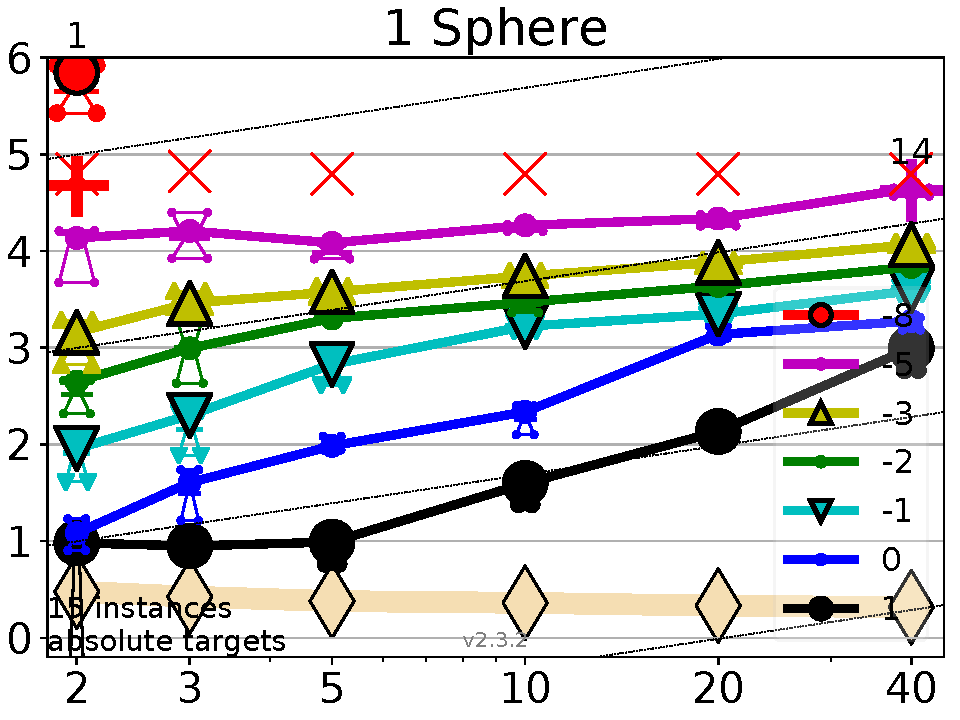
\includegraphics[width=0.28\textwidth]{GAOnly_f001}&
    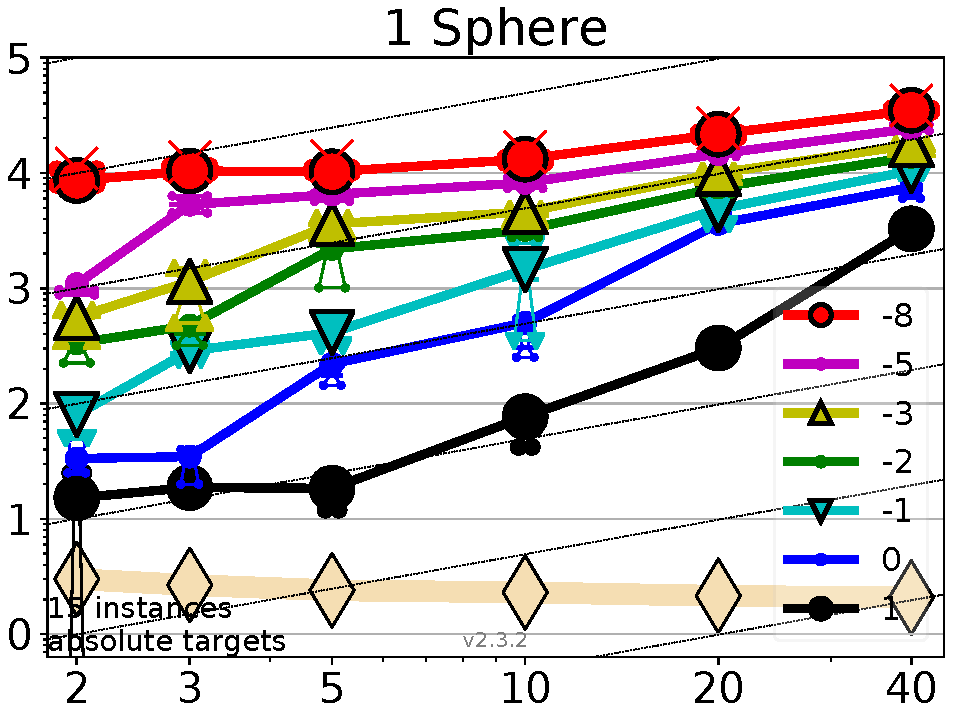
\includegraphics[width=0.28\textwidth]{PSOOnly_f001}&
    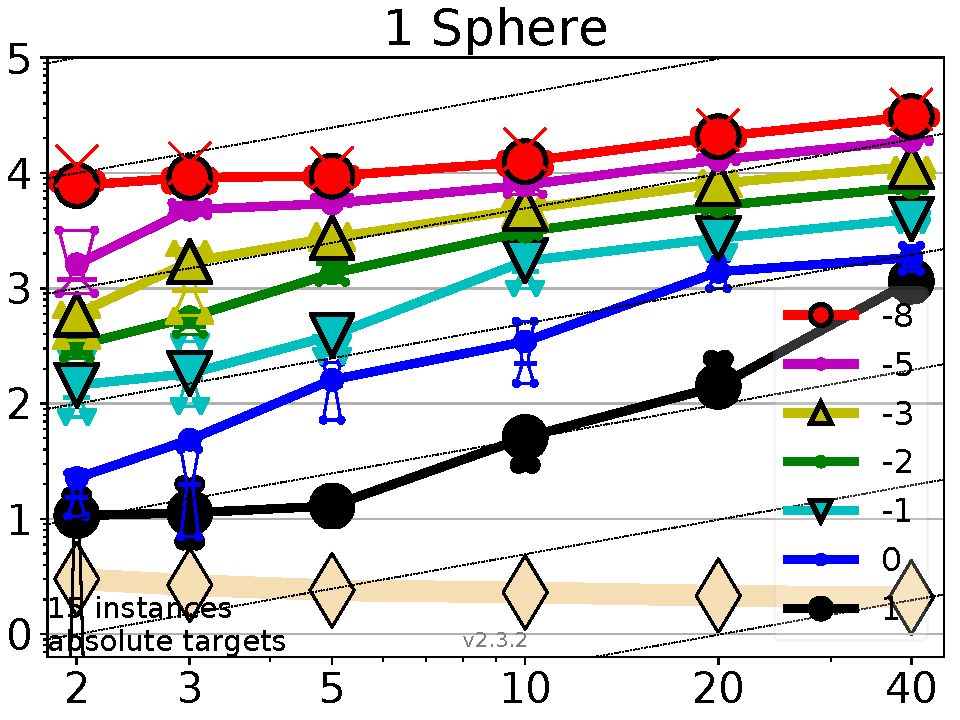
\includegraphics[width=0.28\textwidth]{GAPSO_f001}\\

    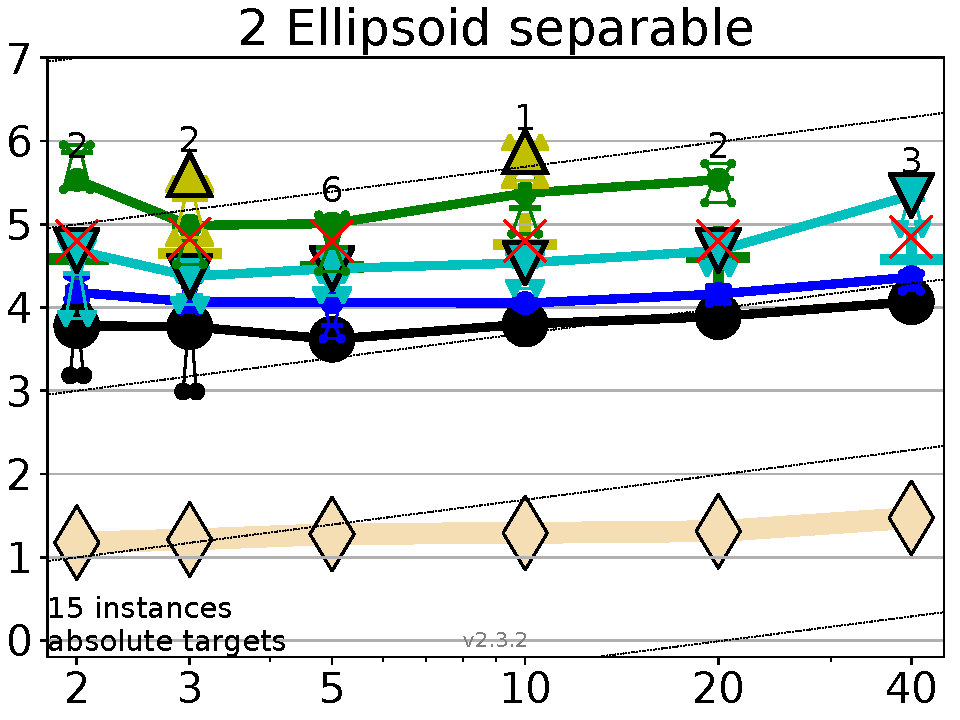
\includegraphics[width=0.28\textwidth]{GAOnly_f002}&
    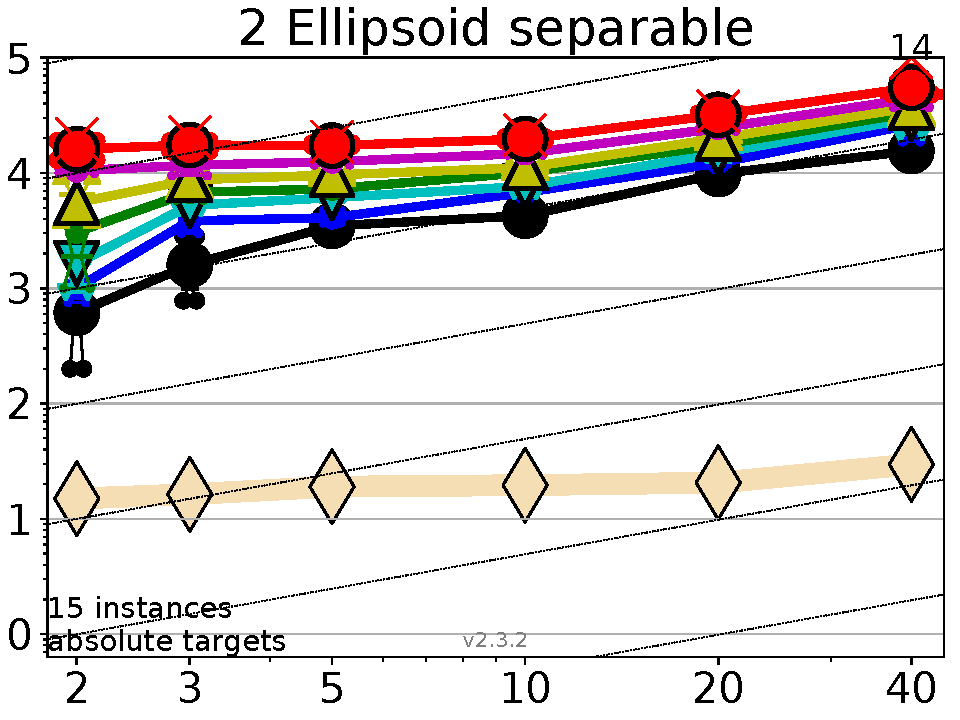
\includegraphics[width=0.28\textwidth]{PSOOnly_f002}&
    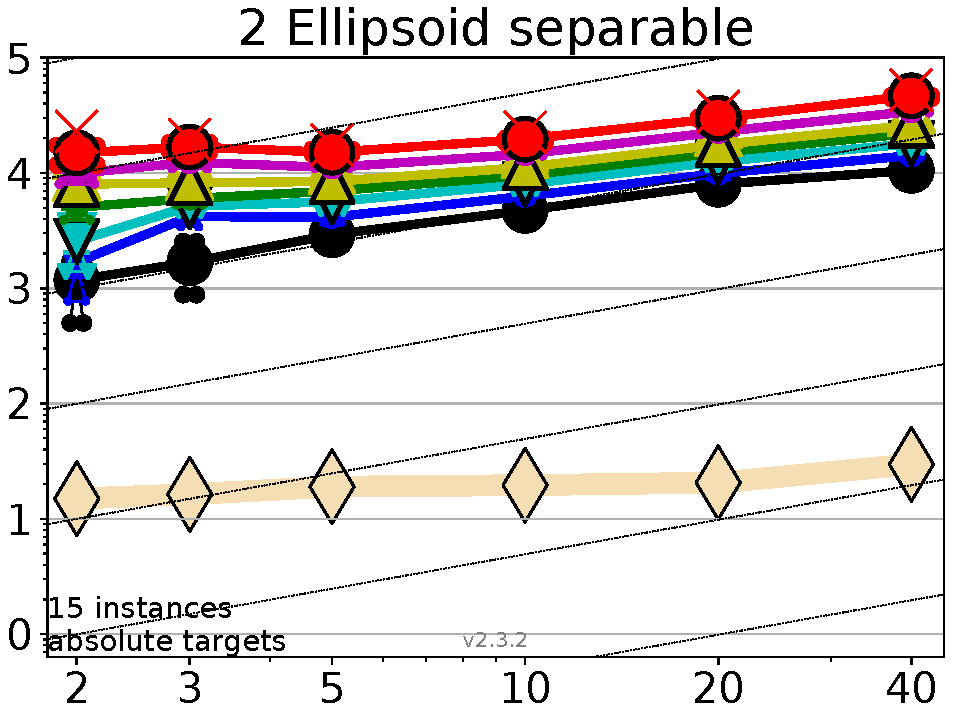
\includegraphics[width=0.28\textwidth]{GAPSO_f002}\\

    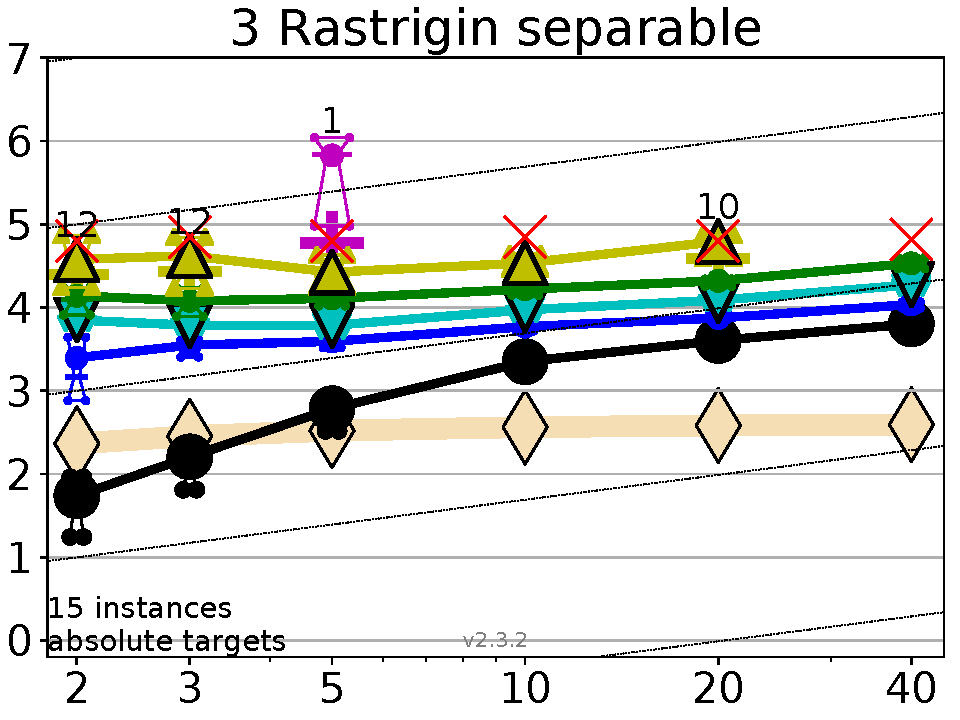
\includegraphics[width=0.28\textwidth]{GAOnly_f003}&
    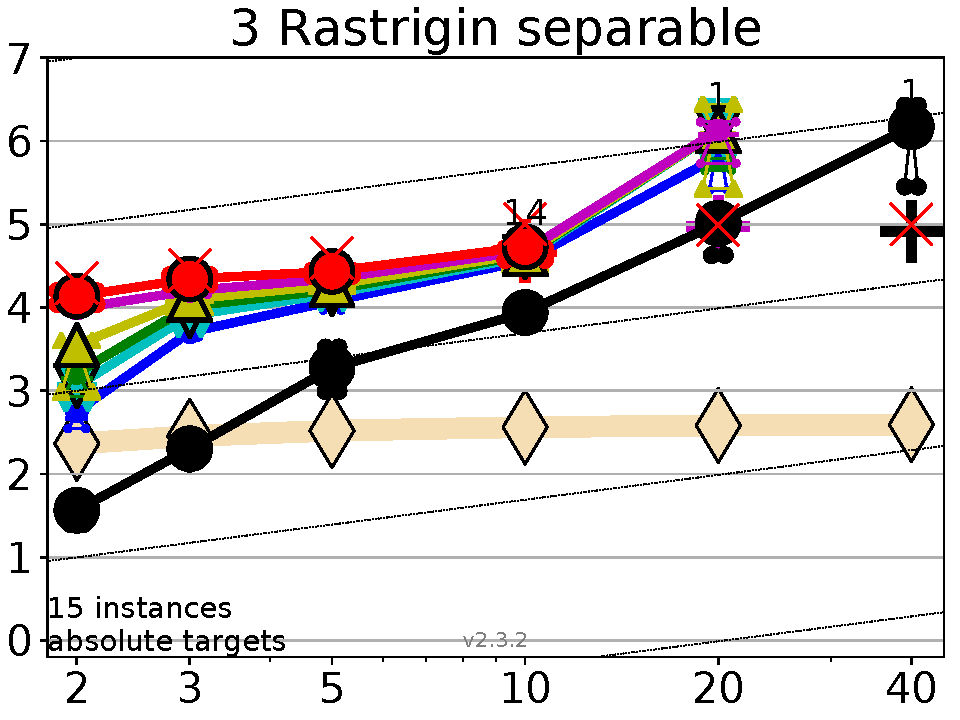
\includegraphics[width=0.28\textwidth]{PSOOnly_f003}&
    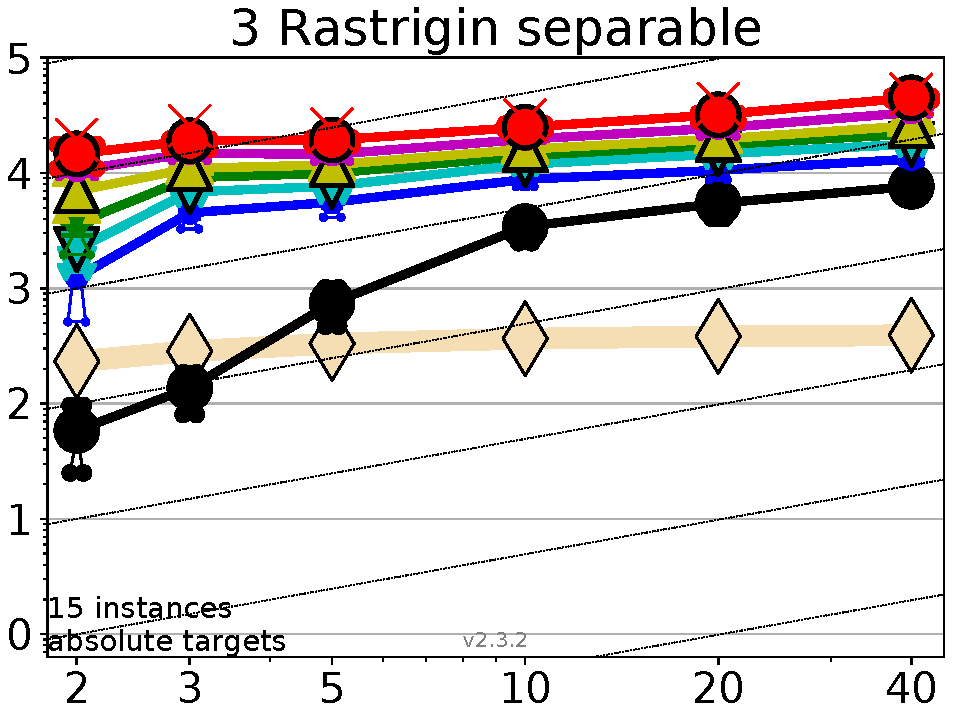
\includegraphics[width=0.28\textwidth]{GAPSO_f003}\\

    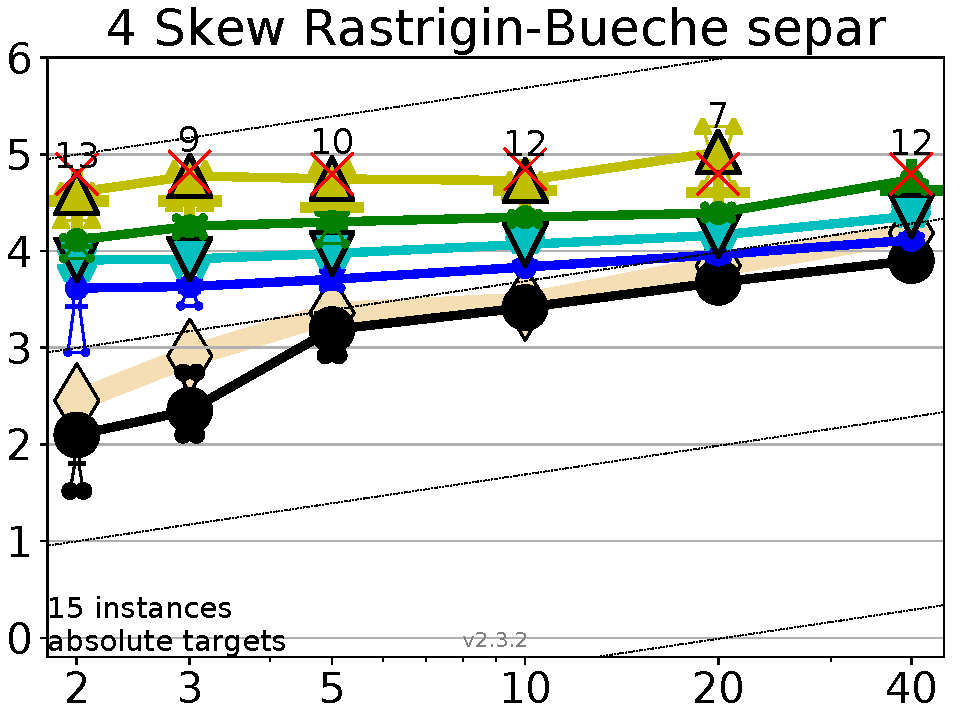
\includegraphics[width=0.28\textwidth]{GAOnly_f004}&
    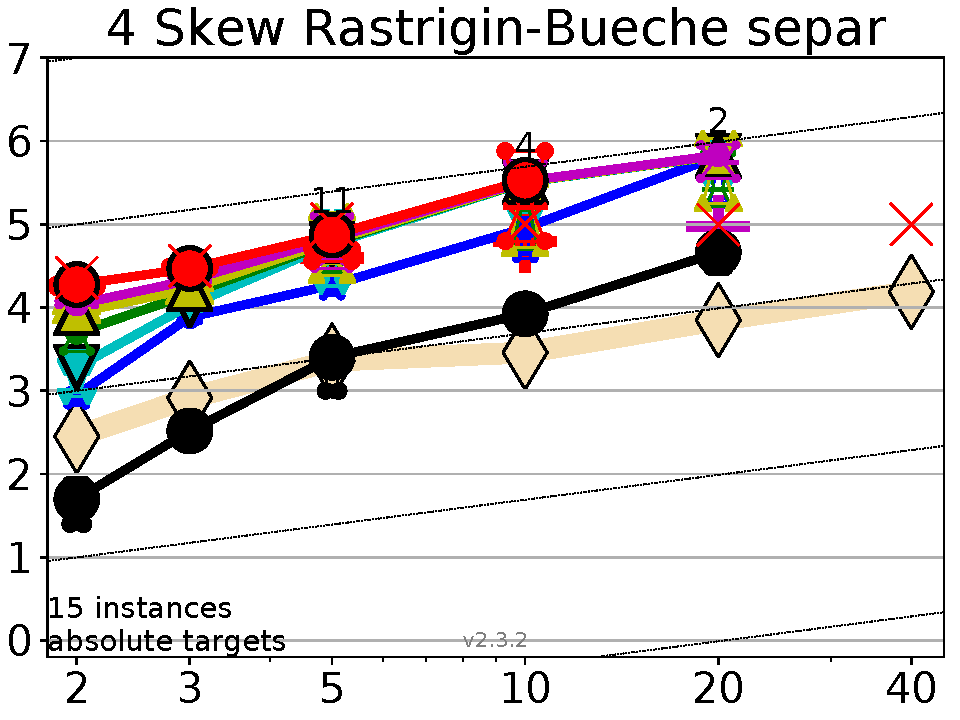
\includegraphics[width=0.28\textwidth]{PSOOnly_f004}&
    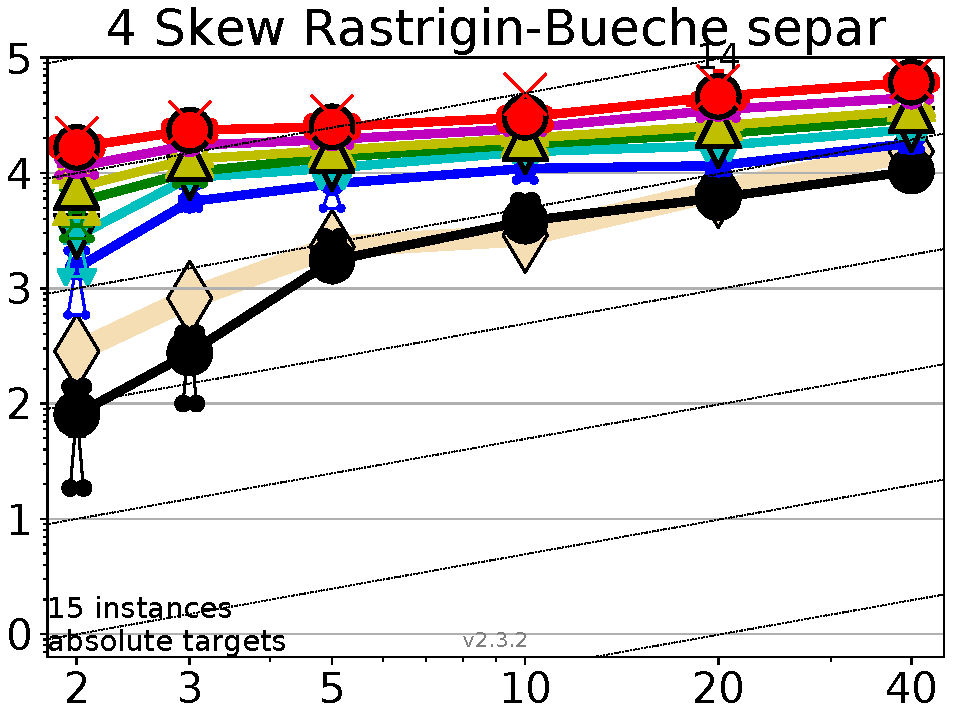
\includegraphics[width=0.28\textwidth]{GAPSO_f004}\\

    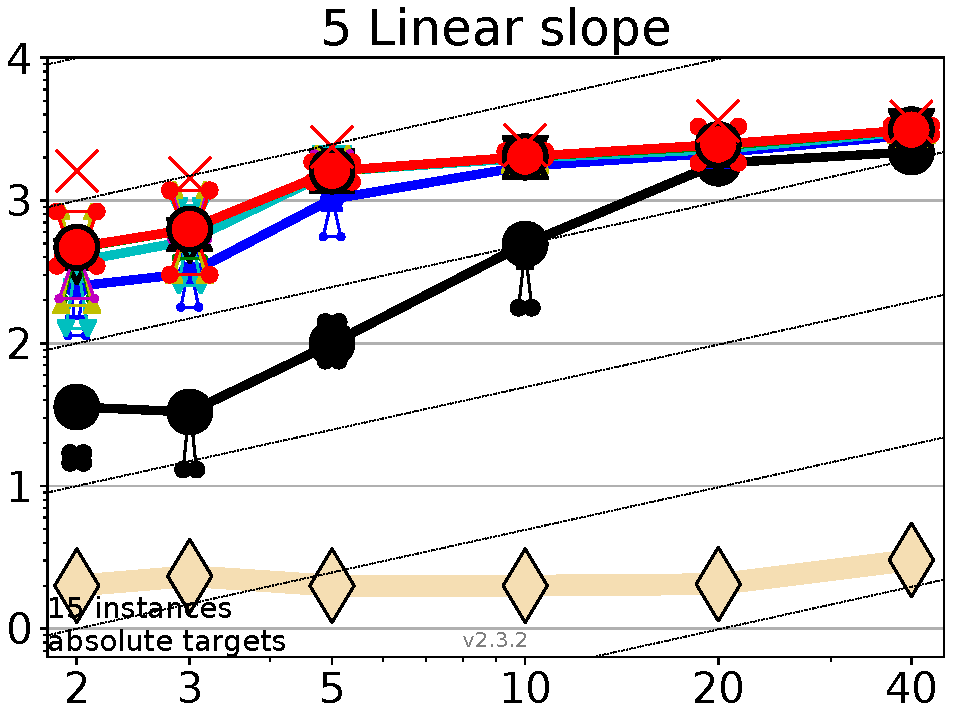
\includegraphics[width=0.28\textwidth]{GAOnly_f005}&
    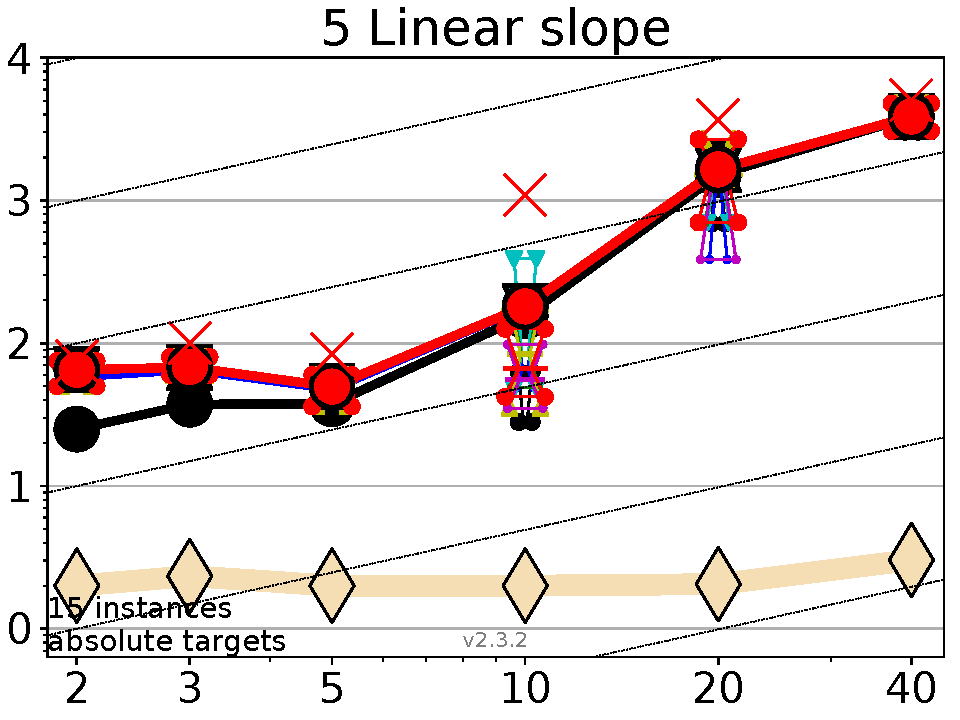
\includegraphics[width=0.28\textwidth]{PSOOnly_f005}&
    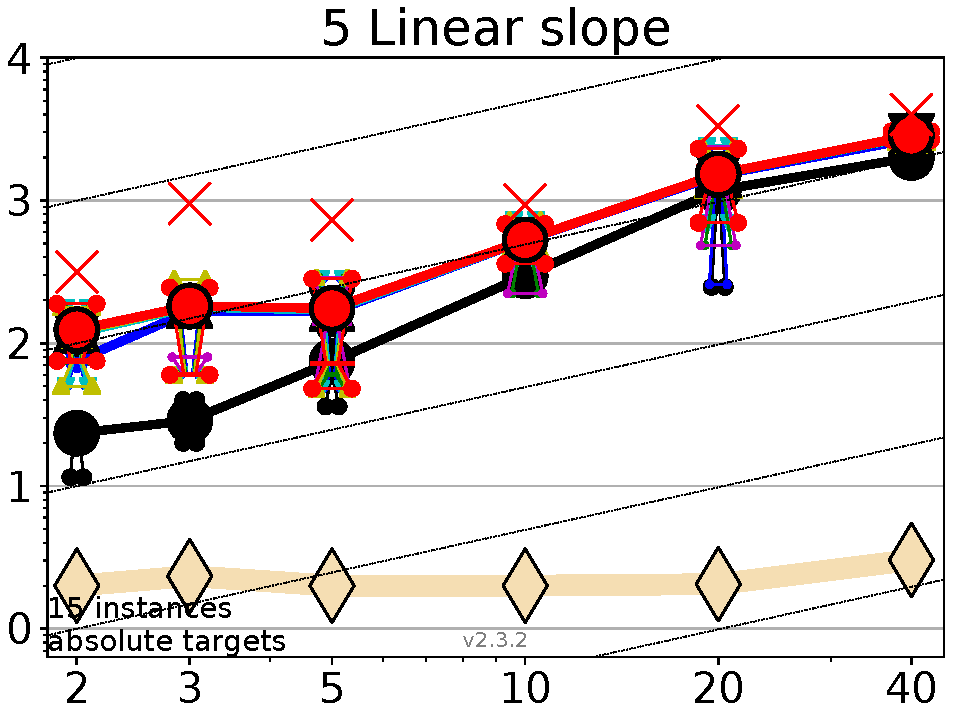
\includegraphics[width=0.28\textwidth]{GAPSO_f005}\\
    \end{tabular}
    \vspace{-3ex}
     \caption{
 Scaling of running time with problem dimension to reach certain target values $\Delta f$. Lines:
 average runtime (aRT); Cross ($+$): median runtime of successful runs to reach
 the most difficult target that was reached at least once (but not always);
 Cross (\textcolor{red}{$\times$}): maximum number of f-evaluations in any trial. Notched boxes:
 interquartile range with median of simulated runs; all values are divided by
 dimension and plotted as $log_{10}$ values versus dimension. 
 %Shown is the aRT for
 %fixed values of $\Delta f = 10k$ with $k$ given in the legend. 
 %Numbers above aRT-symbols
 %(if appearing) indicate the number of trials reaching the respective target.
 %The light thick line with diamonds indicates the best algorithm from BBOB 2009
 %for the most difficult target. Horizontal lines mean linear scaling, slanted
 %grid lines depict quadratic scaling.
}
\label{fig:bbob}
\end{figure*}


\begin{figure*}[h!tb]
  \begin{tabular}
      {c@{\hspace*{-0.00001\textwidth}}
       c@{\hspace*{-0.00001\textwidth}}
       c@{\hspace*{-0.00001\textwidth}}
      }
  10D &  20D & 40D\\   
  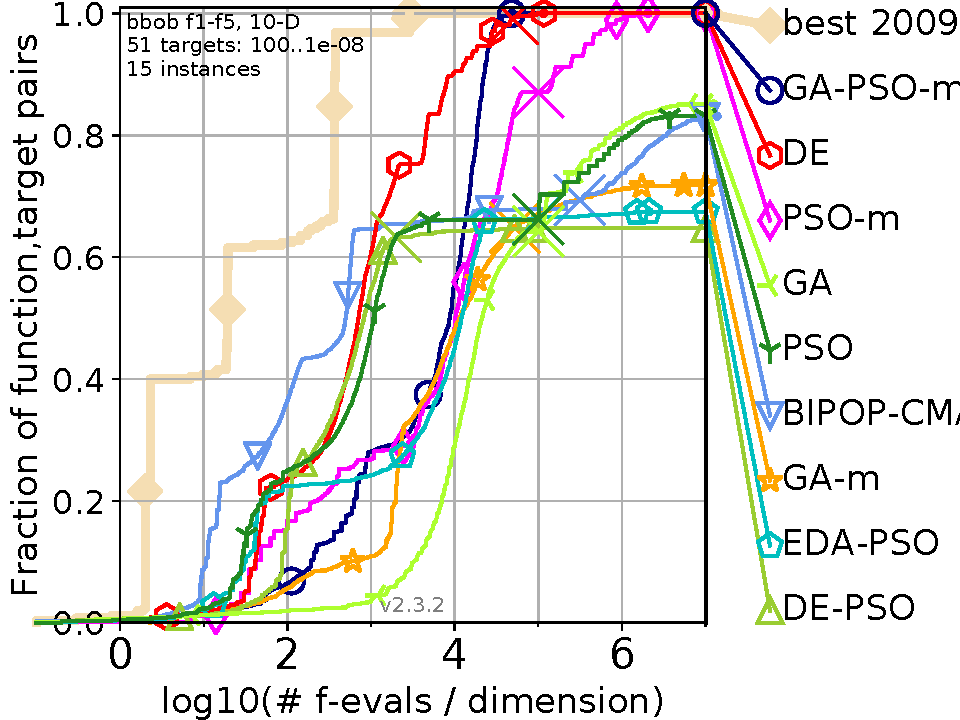
\includegraphics[width=0.30\textwidth]{pprldmany_10D_separ}&
  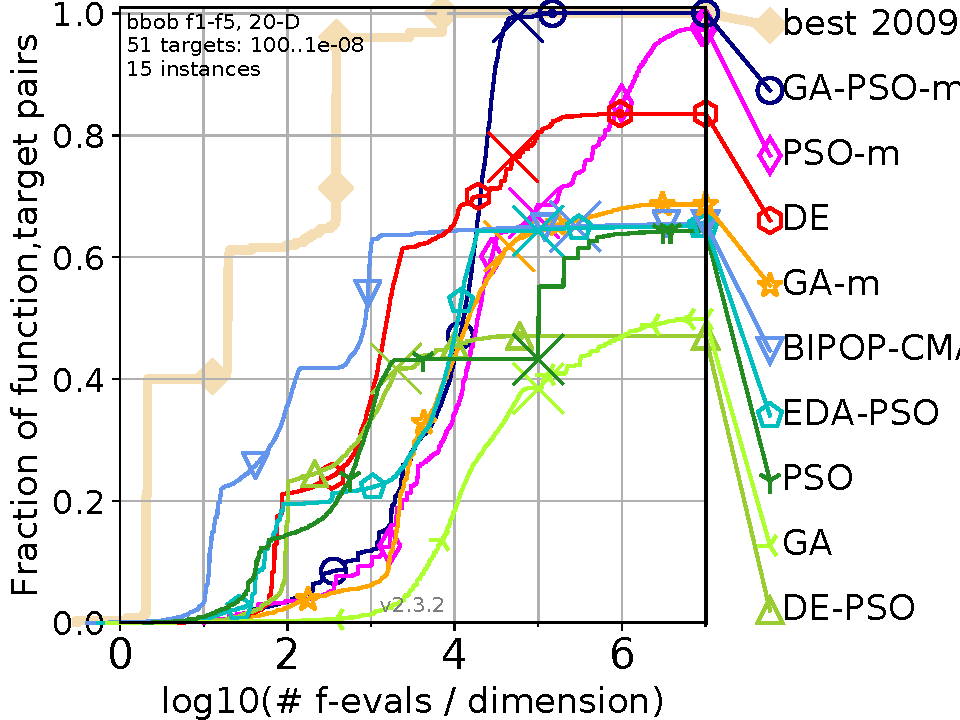
\includegraphics[width=0.30\textwidth]{pprldmany_20D_separ}&
  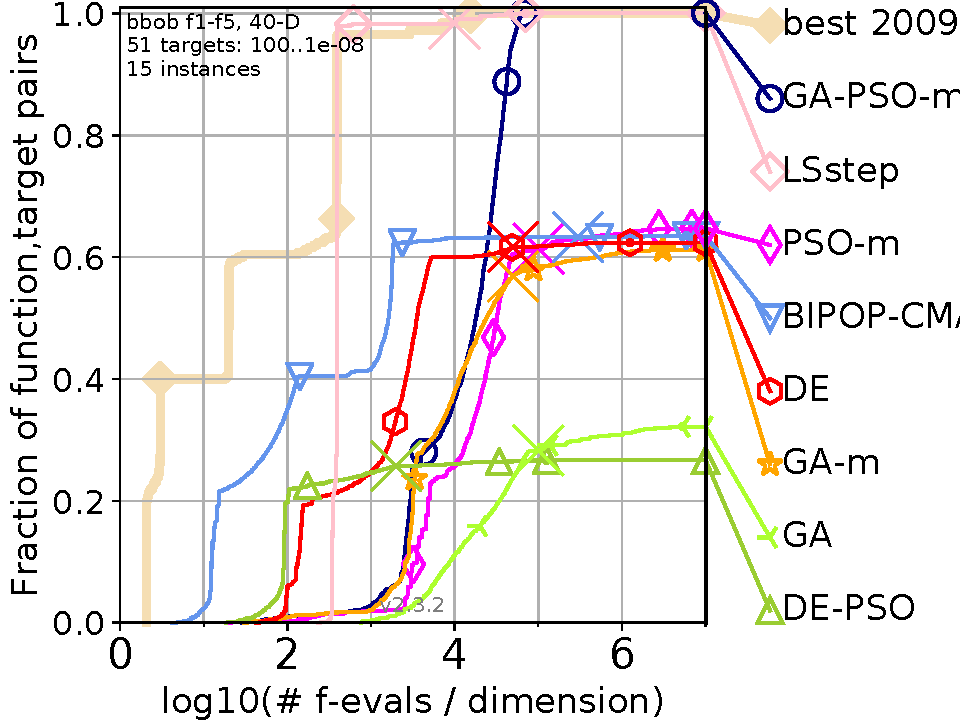
\includegraphics[width=0.30\textwidth]{pprldmany_40D_separ}\\

\end{tabular} \vspace{-3ex} \caption{ Bootstrapped empirical cumulative
distribution of the number of objective function evaluations divided by
dimension (FEvals/DIM) for separable functions.  
 } \label{fig:bbob2} 
\end{figure*}






\section{Conclusions and future lines of work}
\label{conclusions}

In this paper we have presented a new multi-population, hybrid,
stateless bioinspired algorithm that uses different processing units to
evolve sets of populations, which behave as a stream of continuously
updated messages. Population and evolution (or any other kind of
change) are totally decoupled, and its processing is stateless, which
makes possible to create a mixture of processing algorithms that work
asynchronously and in a way that's totally independent of each other.

We have tested this combination of algorithms on the BBOB benchmark
functions, obtaining results that are better that those obtained by
any of them separated. This confirms results obtained by previous
authors in hybrid algorithms, except that, in this case, the architecture is different and
there are improvements all across the tested functions; besides,
results are better than results that have been published for other
algorithms, including a hybrid one, making the hybrid PSO/GA a firm
contender in the function optimization arena. % Probably add a bit of more stuff here, like ...
It is interesting to note that this is done despite mixing both
algorithms in a totally random way, so that it's really impossible to
know whether an individual population will be processed by a GA or
PSO, or how many cycles of each has undergone. The migration process,
however, guarantees a mixing of results and is probably the key to the
ultimate success of the algorithm proposed here. % Check that this
                                % seems reasonable - JJ

As future lines of work, we will try to add different
population-based, data-compatible algorithms to the mix, to see what
kind of results they obtain and what could possible be the best
possible mix. A way of automatically scaling to get the number of
nodes needed would also be a very interesting feature.

An extensive study on the real effects of the mix of algorithms should
also be performed, with a theoretical basis if possible, using the
size of the basins of attractions, for instance, or how different
algorithms move along the fitness landscape.


\section*{Acknowledgments}
The authors would also like to thank the anonymous referees for
their valuable comments and helpful suggestions. The work is
supported by the so and so.





%
% the environments 'definition', 'lemma', 'proposition', 'corollary',
% 'remark', and 'example' are defined in the LLNCS documentclass as well.
%

%
% ---- Bibliography ----
%
% BibTeX users should specify bibliography style 'splncs04'.
% References will then be sorted and formatted in the correct style.
%
\bibliographystyle{splncs04}
\bibliography{multipopulation,hybrid} 

\end{document}
